\documentclass{beamer}
\usepackage[utf8]{inputenc}
\usepackage{graphicx} %package to manage images
% \graphicspath{ {./images/chapter8} }
\usepackage{amsmath}
\usetheme{Berlin}
%\usecolortheme{beaver}
% Information to be included in the title page:
\title{Schottky Barrier Diode}
\subtitle{Chapter 8}
\author{Bonface~K.~M. \and Kanyi~Naftary}
\institute{
  Department of Electrical and Electronic Engineering \\
  University of Nairobi
}
\date{October 2017}

\begin{document}

\frame{\titlepage}
\begin{frame}
  \frametitle{Table of Contents}
  \tableofcontents
\end{frame}

%%%%%%%%%%%%%%%%
% Introduction %
%%%%%%%%%%%%%%%%
\section{Introduction}
\begin{frame}
  \frametitle{Introduction}
  % What are schottky barrier diodes?
  Schottky Barrier Diodes are metal semi-conductor junctions having rectifying properties.
  % Where are they used?
  They are used as detectors and mixers at microwave frequencies (we shall explore later why this is so).
\end{frame}



%%%%%%%%%%%%%%%%%%%%%%%
% Theory of operation %
%%%%%%%%%%%%%%%%%%%%%%%
\section{Theory}
\begin{frame}
  \frametitle{Theory}
  \framesubtitle{Definitions}
  $ e\phi_m$: work function of a metal, is the energy required for removal of an electron in metal from its Fermi-level to the outside vacuum.

  $e\phi_s$: work function of a semiconductor, is the energy required for removal of an electron in semiconductor from its Fermi-level to the outside vacuum.

  $e\chi$: electron affinity, is the energy required to lift an electron from the lowest level of conduction band to vacuum level.
\end{frame}

\begin{frame}
  \begin{figure}[h]
    \caption{Metal-semiconductor band diagrams before contact}
    \centering
    \includegraphics[width=0.4\textwidth]{./images/chapter8/fig8_1.png}
    \label{fig:8_1}
  \end{figure}

  After contact in figure \ref{fig:8_1}, the electron energy in the semiconductor must be lowered relative to the electron energy in the metal. This has the effect of creating a thin sheet of negative charge on metal side of junction and a depletion region of width \textit{w} on the semiconductor side consisting of immobile positive donor ions as shown in fig \ref{fig:8_2}
\end{frame}

\begin{frame}
  \begin{columns}
    \column{0.5\textwidth}
    \begin{figure}[h]
      \caption{Schottky barrier is a depletion layer formed at the junction of a metal and a semiconductor}
      \centering
      \includegraphics[width=0.7\textwidth]{./images/chapter8/fig8_2.png}
      \label{fig:8_2}
    \end{figure}

    \column{0.8\textwidth}
    \begin{figure}[h]
      \caption{Schottky barrier energy band diagram after contact at equilibrium}
      \centering
      \includegraphics[width=0.4\textwidth]{./images/chapter8/fig8_3.png}
      \label{fig:8_3}
    \end{figure}
  \end{columns}

  In figure \ref{fig:8_3}, the $e\phi_b$ is called the \emph{barrier height}.
  $e\phi_b = e\phi_m - e\chi$
  The voltage drop across the depletion layer \emph{w} of the semiconductor is called the \emph{equilibrium contact potential} $V_{bi}$. It prevents further diffusion of electrons from the conduction band of the semiconductor to the metal.
\end{frame}

\begin{frame}
  The current flowing through a schottky barrier diode is caused by:
  \begin{itemize}
  \item $I_o$ due to electron emission from metal to semiconductor junction over the barrier $(\phi_m - \chi)$
  \item Electron flow from semiconductor conduction band over the contact potential into the metal.
  \end{itemize}

  It can be shown that:
  \[ \phi_b \propto \exp \left(- \frac{e\phi_b}{RT}\right) \]
  \[ \therefore I_0 \propto \exp \left(- \frac{e\phi_b}{RT}\right) \]
\end{frame}

\begin{frame}
  For flow of current from semiconductor to metal, it is to be noted that the contact potential difference is reduced to $V_{bi} - V$ for forward bias and is increased to $V_{bi} + V$ for reverse bias. \emph{In forward bias, there is larger electron flow from semiconductor to metal.}
  The diode equation is similar to the diode equation for p-n junction which has the form:
  \[ I = A \exp \left(\frac{-e\phi_b}{kT}\right) \left( \exp \frac{-eV}{kT} -1 \right) \]
\end{frame}

\begin{frame}
  In Schottky Barrier Diodes, the forward current flows due to majority carriers from semiconductor to metal and there is no minority carrier current injection. Hence the phenomena of storage and recombination of minority carriers along with associated time delays do not occur in rectifying Schottky Barrier Diodes (unlike p-n junction rectifiers). Thus very fast switching can take place and the devices are very suitable for detection of high frequency signals.
\end{frame}



%%%%%%%%%%%%%%%%%%
% Surface States %
%%%%%%%%%%%%%%%%%%
\section{Surface States In Practical Schottky Barrier Diodes}
\begin{frame}
  \frametitle{Surface States In Practical Schottky Barrier Diodes}
  The barrier height in a practical barrier Schottky diode differs from an ideal case. In practice, Schottky Barrier Diodes involve a termination of crystal semiconductor lattice at the metal semiconductor boundary. The termination leads to production of surface states due to incomplete covalent bonds which affect the barrier height. There is also a thin layer of $SiO_2$ which also affects the barrier height. \emph{Because of this, for design of Schottky diodes, measured barrier height data is used as opposed to ideal values based on the work function of the isolated metal and semiconductor.}
\end{frame}



%%%%%%%%%%%%%%%%%%%%%%%%%%%%%%%%%
% Structures of schottky diodes %
%%%%%%%%%%%%%%%%%%%%%%%%%%%%%%%%%
\section{Structures Of Schottky Diodes}
\begin{frame}
  \frametitle{Structures of Schottky Diodes}
  2 structures of the schottky diodes are finding wide applications:
  \begin{itemize}
  \item Microwave detection and mixing
  \item Integrated circuits
  \end{itemize}
\end{frame}

\begin{frame}
  \begin{figure}[h]
    \caption{Small area Microwave Schottky diode detector}
    \centering
    \includegraphics[width=0.5\textwidth]{./images/chapter8/fig8_6.png}
    \label{fig:8_6}
  \end{figure}
  A small area semiconductor diode formed by depositing metal by planar process on an epitaxail or $n^+$ substrate is used. The series resistance and the diode capacitance have to be minimized for good performance. The cut-off frequency for forward bias is given by:
  $f_c = \frac{1}{2\pi R_{f}C_f}$ where $R_f$ and $C_f$ are values for forward bias of 0.1 V
\end{frame}
\begin{frame}
  \begin{figure}[h]
    \caption{Metal overlap Schottky structure}
    \centering
    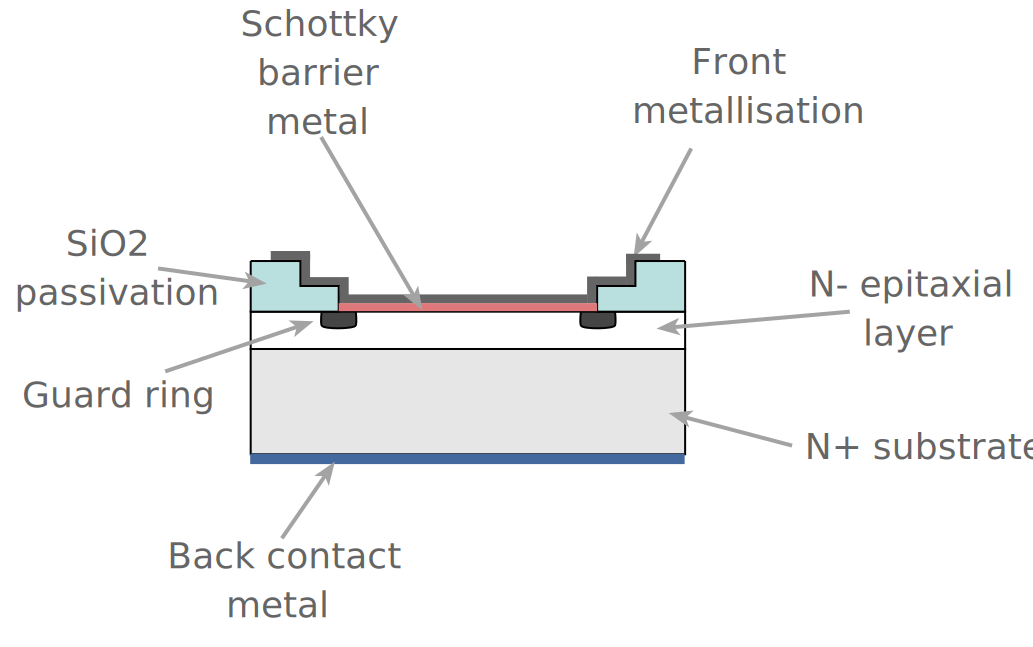
\includegraphics[width=0.4\textwidth]{./images/chapter8/fig8_8.png}
    \label{fig:8_8}
  \end{figure}
  This structure is well suited for integrated circuits. It gives a well forward I-V characteristic and low leakage current. The metal semiconductor junction will behave as an ohmic contact when the semiconductoris highly doped. The heavily doped surface can be formed by shallow diffusion or alloy regrowth.
\end{frame}

\begin{frame}
  The heavily doped layer in the metal semiconductor junction leads to extremely thin a depletion layer. The carriers can tunnel easily through this thin depletion layer from semiconductor to metal and the diffusion of the carriers can tunnel easily through this thin depletion layer from semiconductor to metal and the diffusion of the carriers over the contact potential plays a minor role.  Thus current flows through tunnelling of the electrons from the semiconductor to the metal irrespective of the polarity of the bias voltage. Thus current can flow in both the directions making the metal semiconductor junction behave like an ohmic contact.

\end{frame}
\end{document}